\documentclass[reprint,amsmath,amssymb,aps,prd,floatfix]{revtex4-2}

% === Core formatting ===
\usepackage[english]{babel}
\usepackage{graphicx}
\usepackage{dcolumn}
\usepackage{bm}
\usepackage{ragged2e}
\usepackage{enumitem}
\usepackage{booktabs}
\usepackage{multirow}
\usepackage{array}
\usepackage{tabularx}
\newcolumntype{Y}{>{\centering\arraybackslash}X}

% === Figures ===
%\usepackage[compatibility=false]{subcaption}
\usepackage{placeins}
\usepackage{adjustbox}

% === Editing tools (remove before submission) ===
\usepackage{comment}
\usepackage[normalem]{ulem}
% \usepackage{lineno}

% === Bibliography style ===
\bibliographystyle{apsrev4-2}

% === Must be near last ===
\usepackage[hidelinks,colorlinks=true,linkcolor=blue,citecolor=blue,urlcolor=blue]{hyperref}
\usepackage{bookmark}
\usepackage{cleveref}

% === Custom commands ===
\makeatletter
\newcommand*{\rom}[1]{\expandafter\@slowromancap\romannumeral #1@}
\makeatother

\renewcommand{\topfraction}{0.9}
\renewcommand{\bottomfraction}{0.9}
\renewcommand{\textfraction}{0.05}
\renewcommand{\floatpagefraction}{0.8}

\begin{document}

\preprint{APS/123-QED}

\title{Comparative study of jet-substructure quark/gluon discriminants in photoproduction at the EIC and HERA}

\author{Siddharth Narayan Singh}
\email{siddharthsingh@brandeis.edu}
\affiliation{Brandeis University, Waltham,~US}

\author{R.~Aggarwal}
\email{ritu.aggarwal1@gmail.com}
\affiliation{USAR and USBAS, Guru Gobind Singh Indraprastha University, East Delhi Campus, 110092, India}

\author{M.~Kaur}
\email{manjit@pu.ac.in}
\affiliation{Department of Physics, Panjab University, Chandigarh 160014, India\\Department of Physics, Amity University, Punjab, Mohali 140306, India}

\date{\today}

\begin{abstract}
\centering \textbf{Abstract}
\begin{justify}
We compare three jet-substructure quark/gluon discriminators in $ep$ photoproduction --- the integrated jet shape $\Psi(r=0.3)$, the $k_T$ exclusive subjet multiplicity $n_{\mathrm{subjets}}$, and the iterated soft-drop multiplicity $n_{\mathrm{SD}}$ --- on identical anti-$k_T$ jets from PYTHIA~8 events at $\sqrt{s} = 64$--$300$~GeV, spanning the EIC design energies and a HERA reference. The integrated jet shape separates gluon from quark jets best at every energy, with ROC areas of $0.75$--$0.77$ against $0.66$--$0.69$ for $n_{\mathrm{SD}}$ and $0.53$--$0.65$ for $n_{\mathrm{subjets}}$, the last degrading with $\sqrt{s}$ as pooling over pseudorapidity dilutes it. Carrying no internal tagging parameters and directly comparable to archival HERA data, the integrated jet shape is well matched to first-generation EIC measurements.
\end{justify}
\end{abstract}

\maketitle

% \tableofcontents

\section{Introduction}\label{sec:intro}

The classification of jets by the flavor of the initiating parton, quark or gluon, is one of the most studied problems in jet substructure. The two classes differ in radiation pattern at the leading-log level by the ratio of color Casimirs, $C_A / C_F = 2.25$ in QCD, and many physical observables built from the jet's internal energy and angular distributions inherit some fraction of this discrimination power. The literature on quark/gluon taggers spans several decades: from early measurements at LEP and HERA based on jet-shape variables and subjet multiplicities, through theoretically motivated grooming observables such as iterated soft-drop multiplicity, generalised angularities and energy-flow polynomials, and most recently to deep-learning approaches that operate directly on the jet's constituents. The questions of which observable is ``best'' and what ``best'' should even mean depend strongly on the experimental setting, collision system, kinematic range, available statistics, and the relative weight given to interpretability versus raw tagging power.

The Electron-Ion Collider~(EIC), currently under construction at Brookhaven National Laboratory, will provide an unprecedented testing ground for jet substructure in a cleaner environment than $pp$ colliders. In particular, $ep$ photoproduction at the EIC populates a kinematic regime characterised by lower jet transverse energies than at HERA, a substantial admixture of direct and resolved photon processes that varies smoothly with $\sqrt{s}$, and a relatively low underlying-event activity compared with $pp$ collisions. These features make photoproduction at the EIC an attractive setting both for studying jet substructure in its own right and for benchmarking discriminators that will later be applied to higher-multiplicity environments. At the same time, the EIC is a future facility: no measured data exist yet, and any methodological choice that introduces analysis-specific tuning has to be defended without recourse to data-driven calibration.

In this paper we revisit the quark/gluon tagging question in the specific context of EIC photoproduction. We compare three substructure observables, the integrated jet shape $\Psi(r)$, the $k_T$ exclusive subjet multiplicity $n_{\mathrm{subjets}}$, and the iterated soft-drop multiplicity $n_{\mathrm{SD}}$, on the same jets, reconstructed in the same way, across four center-of-mass energies spanning HERA and the three EIC design energies. Our motivation is twofold. First, the integrated jet shape is the observable used in our recent photoproduction study, where it is the basis for the thin/thick classifier that produces the quark- and gluon-enriched jet samples reported there. The choice was historically motivated by direct comparability with the published HERA-ZEUS data, but its quantitative performance against alternative discriminators in the EIC kinematic regime had not been established. Second, the iterated soft-drop multiplicity is a well-known counting tagger that has been argued to outperform $n_{\mathrm{subjets}}$ on theoretical grounds, its leading-log behaviour approaches the $C_A / C_F$ Casimir ratio per hard splitting. Verifying whether this advantage holds empirically in the soft, low-$E_T$ EIC regime, and how it compares to a continuous integrated observable like $\Psi(r)$, is the central question of this work.

We find that the ordering $\Psi(r=0.3) > n_{\mathrm{SD}} > n_{\mathrm{subjets}}$ holds in every sample we examined. The integrated jet shape gives the largest ROC AUC at all four center-of-mass energies, and the advantage of $n_{\mathrm{SD}}$ over $n_{\mathrm{subjets}}$ widens as $\sqrt{s}$ grows from 64~GeV to 300~GeV --- though that ordering reverses once the measurement is binned in pseudorapidity. We give a qualitative physical interpretation of these findings in terms of the integrated-versus-counting nature of the observables, and we discuss the implications for the design of first-generation EIC jet-substructure measurements.

The remainder of this paper is organised as follows. Section~\ref{sec:generation} summarises the event generation and jet reconstruction, with cross-references to the companion paper for full details. Section~\ref{sec:observables} defines the three substructure observables. Section~\ref{sec:roc} specifies the ROC construction and the figures-of-merit (AUC, mean separation, operating-point analysis). Section~\ref{sec:results} presents the per-sample results, the cross-energy trend and the effect of pseudorapidity binning. Section~\ref{sec:discussion} discusses the physical interpretation and the implications for EIC measurements. Section~\ref{sec:conclusion} concludes.

\section{Event generation and jet reconstruction}\label{sec:generation}

We generate events with \textsc{Pythia}~8.312~\cite{10.21468/SciPostPhysCodeb.8}
using asymmetric $ep$ beams. The photon is quasi-real
(\texttt{PDF:beamB2gamma = on}): we require $Q^2 < 1~\mathrm{GeV}^2$, which is
what makes the process photoproduction.
\textsc{Pythia} mixes the direct and resolved contributions on its own
(\texttt{Photon:ProcessType = 0}); \texttt{HardQCD:all} provides the Born
$2\to2$ matrix elements for the resolved photon and \texttt{PhotonParton:all}
those for the pointlike one. We set the multiparton-interaction parameter
$p_{T0}^{\mathrm{ref}} = 3.0$~GeV everywhere.

We simulate four beam setups --- one HERA reference and the three EIC design
energies --- with $10^6$ events each. Table~\ref{tab:samples} lists them.

\begin{table}[htbp]
\caption{Beam configurations and dijet yields. $N_{\mathrm{QQ}}$ and
$N_{\mathrm{GG}}$ count jets, not events, after the full selection described in
the text.}
\label{tab:samples}
\begin{ruledtabular}
\begin{tabular}{cccccc}
$\sqrt{s}$ & $E_p$ & $E_e$ & $\hat{p}_T^{\min}$ & $N_{\mathrm{QQ}}$ & $N_{\mathrm{GG}}$ \\
$[\mathrm{GeV}]$ & [GeV] & [GeV] & [GeV] & & \\
\colrule
 63.2 & 100 & 10.0 & 5 &  15\,132 &    758 \\
104.9 & 275 & 10.0 & 5 &  25\,258 &  2\,796 \\
140.7 & 275 & 18.0 & 7 & 135\,800 & 22\,930 \\
300.3 & 820 & 27.5 & 7 & 134\,774 & 57\,592 \\
\end{tabular}
\end{ruledtabular}
\end{table}

We label each event by the flavours of the two outgoing partons of the hard
$2\to2$ process, which we read straight from the \textsc{Pythia} process code.
Two outgoing quarks (codes 112, 114, 116, 121--124 for the resolved photon;
271--273 and 281--283 for boson--gluon fusion) give QQ; two outgoing gluons
(111, 115) give GG; one of each (113 for the resolved photon; 274 and 284 for
QCD Compton) gives GQ. We checked every generated event: the labelling is
self-consistent to better than $99.99\%$ in all four samples, with only
$\mathcal{O}(10)$ events per sample leaking in from process 284. We use QQ and
GG as the two classes to separate. A GQ event contains one jet of each flavour,
so its jets carry no class label of their own, and we drop them.

We build jets with \textsc{FastJet}~3~\cite{Cacciari_2012} using
anti-$k_T$~\cite{Cacciari:2008gp} at $R = 1.0$. A final-state particle joins the
clustering if $p_T > 0.1$~GeV and $|\eta| < 5$. We keep events with exactly two
jets in $-4 < \eta < 4$, the leading jet above $E_T = 10$~GeV and the subleading
one above $7$~GeV. Asking for exactly two jets removes events with extra hard
radiation between the jet directions, which in boson--gluon fusion can come from
colour exchange between the outgoing partons.

One point matters more than any other here: \emph{all three observables are
computed on the same jets, in the same event loop}. Same jet definition, same
cuts, same $E_T$ thresholds, at all four energies. Every jet gives a matched
triplet $(\Psi(0.3),\,n_{\mathrm{SD}},\,n_{\mathrm{subjets}})$, so any
difference in performance between the three comes from the observables
themselves and not from the samples or the reconstruction.

\section{Substructure observables}\label{sec:observables}

\subsection{Integrated jet shape $\Psi(r)$}

The integrated jet shape is the average fraction of a jet's transverse energy
that falls inside a cone of radius $r$ around the jet axis,
\begin{equation}
\Psi(r) \;=\; \frac{1}{E_T^{\mathrm{jet}}}
\sum_{i \,\in\, \mathrm{jet}} E_{T,i}\;\Theta\!\left(r - \Delta R_i\right),
\label{eq:psi}
\end{equation}
where $\Delta R_i = \sqrt{(\Delta\eta_i)^2 + (\Delta\phi_i)^2}$ is how far
constituent $i$ sits from the jet axis and $\Theta$ is the step function. By
construction $\Psi(R) = 1$. We read $\Psi$ at $r = 0.3$, the working point of the
companion analysis and the value the archival ZEUS measurements are quoted
at~\cite{zeus1998measurement,Chekanov_2008,chekanov2008three}.

Quark jets are more collimated than gluon jets of the same $E_T$, so they have
the larger $\Psi(0.3)$. The other two observables run the other way, larger for
gluons, so we build the ROC for $\Psi$ from $-\Psi(0.3)$ and keep one convention
throughout.

$\Psi(r)$ has no threshold anywhere in it. Every constituent contributes,
weighted by its transverse energy, and nothing is thrown away.

\subsection{Exclusive $k_T$ subjet multiplicity}

We recluster the constituents of each anti-$k_T$ jet with the
longitudinally-invariant $k_T$ algorithm~\cite{Catani:1993hr} at the same
$R = 1$, using the pair distance
$d_{ij} = \min(p_{T,i}^2, p_{T,j}^2)\,\Delta R_{ij}^2/R^2$. We stop once every
remaining pair has $d_{ij} > y_{\mathrm{cut}}\,Q^2$, and $n_{\mathrm{subjets}}$
is how many proto-jets are left. We take $y_{\mathrm{cut}} = 5\times10^{-4}$,
the HERA convention, so the result can be compared with the archival data.

The catch is that $y_{\mathrm{cut}}Q^2$ is an \emph{absolute} momentum scale,
about $0.2~\mathrm{GeV}^2$ for a 20~GeV jet. Hard perturbative splittings pass
it, but so does soft wide-angle radiation. Section~\ref{sec:results} shows what
this costs.

\subsection{Iterated soft-drop multiplicity}

The iterated soft-drop multiplicity~\cite{Frye:2017yrw} counts how many
splittings along the jet's primary branch pass a momentum-fraction cut,
\begin{equation}
n_{\mathrm{SD}}(z_{\mathrm{cut}},\beta) \;=\;
\sum_{i \,\in\, \mathrm{primary}}
\Theta\!\left[\, z_i - z_{\mathrm{cut}}
\left(\frac{\Delta R_i}{R_0}\right)^{\!\beta} \,\right],
\label{eq:nsd}
\end{equation}
where a splitting into prongs $(p_1, p_2)$ with $p_{T,1} \ge p_{T,2}$ has
\begin{equation}
z_i \;=\; \frac{p_{T,2}}{p_{T,1} + p_{T,2}}, \qquad
\Delta R_i \;=\; \Delta R(p_1, p_2).
\end{equation}
We recluster the constituents with the Cambridge/Aachen
algorithm~\cite{Dokshitzer:1997in,Wobisch:1998wt} at $R_0 = R$. C/A clusters
purely by angle, so undoing it gives an angle-ordered sequence of splittings ---
the same ordering a coherent QCD shower produces. We then walk the tree from the
root, always following the harder prong, and add one to the counter each time
Eq.~(\ref{eq:nsd}) is satisfied. Unlike the soft-drop
groomer~\cite{Larkoski:2014wba}, we never discard the softer prong and we do not
stop at the first splitting that passes. That is what makes the observable
\emph{iterated}.

We use $z_{\mathrm{cut}} = 0.1$ and $\beta = 0$, so the cut is simply $z > 0.1$
regardless of angle --- the modified mass-drop condition of
Ref.~\cite{Dasgupta:2013ihk}, applied over and over. At leading logarithmic
accuracy the emission density along the primary branch is proportional to the
colour Casimir of the initiating parton, which gives
\begin{equation}
\frac{\langle n_{\mathrm{SD}}\rangle_{\mathrm{gluon}}}
     {\langle n_{\mathrm{SD}}\rangle_{\mathrm{quark}}}
\;\longrightarrow\; \frac{C_A}{C_F} \;=\; 2.25
\label{eq:casimir}
\end{equation}
in the asymptotic limit.

The important difference from $n_{\mathrm{subjets}}$ is that the cut is on the
dimensionless fraction $z$, not on an absolute momentum. At $\beta = 0$,
$n_{\mathrm{SD}}$ therefore barely changes if the jet momentum scale changes.
This one property drives most of what separates the two counting observables
below.

\section{ROC construction and figures of merit}\label{sec:roc}

For a discriminant $X$ with the convention that gluon jets have the larger value,
we take jets from GG events as signal and jets from QQ events as background, and
define for every threshold $c$
\begin{equation}
\varepsilon_{\mathrm{GG}}(c) = \Pr(X \ge c \mid \mathrm{GG}), \qquad
\varepsilon_{\mathrm{QQ}}(c) = \Pr(X \ge c \mid \mathrm{QQ}).
\end{equation}
The ROC curve is what
$\bigl(\varepsilon_{\mathrm{QQ}}(c), \varepsilon_{\mathrm{GG}}(c)\bigr)$ traces
out as $c$ sweeps across the range of $X$. For the two counting observables $c$
runs over integers, so the curve is piecewise linear with one node per cut you
can actually make; for $\Psi(0.3)$ it runs over a fine grid. The area under the
curve,
\begin{equation}
\mathrm{AUC} \;=\; \int_0^1 \varepsilon_{\mathrm{GG}}\,
\mathrm{d}\varepsilon_{\mathrm{QQ}},
\end{equation}
we get by trapezoidal integration over the nodes sorted by increasing
$\varepsilon_{\mathrm{QQ}}$. An AUC of $0.5$ means no discrimination at all and
$1$ means perfect separation.

Alongside the AUC we quote the mean separation
\begin{equation}
\mathcal{S} \;=\;
\frac{\langle X\rangle_{\mathrm{GG}} - \langle X\rangle_{\mathrm{QQ}}}
     {\sqrt{\sigma^2_{\mathrm{QQ}} + \sigma^2_{\mathrm{GG}}}},
\label{eq:sep}
\end{equation}
which only sees the shift in the means, while the AUC also picks up differences
in the shape of the distributions. Comparing the two is useful: if
$\mathcal{S}$ is small but the per-bin AUC is large, the class separation is
being washed out by a spread that carries no class information.

It is worth saying plainly what the ROC adds over the fixed-cut analysis of the
companion paper. There, a jet is called thin if $\Psi(0.3) > 0.8$ and thick if
$\Psi(0.3) < 0.6$, and the purity of the resulting samples is quoted. That is
one operating point. The ROC gives the whole curve, so the purity at any other
working point follows immediately: for starting populations $N_{\mathrm{QQ}}$,
$N_{\mathrm{GG}}$ and $N_{\mathrm{GQ}}$,
\begin{equation}
\mathrm{Purity}_{\mathrm{GG}} =
\frac{N_{\mathrm{GG}}\,\varepsilon_{\mathrm{GG}}}
     {N_{\mathrm{QQ}}\varepsilon_{\mathrm{QQ}}
    + N_{\mathrm{GG}}\varepsilon_{\mathrm{GG}}
    + N_{\mathrm{GQ}}\varepsilon_{\mathrm{GQ}}}.
\end{equation}
Every efficiency and purity quoted here is an ensemble-level number: it is a
fraction within a population of classified jets, not a calibrated probability
for any individual jet.

\section{Results}\label{sec:results}

\subsection{Discriminant ordering}

Figure~\ref{fig:roc_panels} shows the ROC curves for the three observables at each
of the four centre-of-mass energies. The ordering
\begin{equation}
\Psi(r=0.3) \;>\; n_{\mathrm{SD}} \;>\; n_{\mathrm{subjets}}
\end{equation}
holds in every sample. The integrated jet shape reaches AUC values between
$0.745$ and $0.768$, the iterated soft-drop multiplicity between $0.657$ and
$0.688$, and the subjet multiplicity between $0.526$ and $0.652$.
Table~\ref{tab:auc} gives the numbers.

\begin{figure*}[t]
\centering
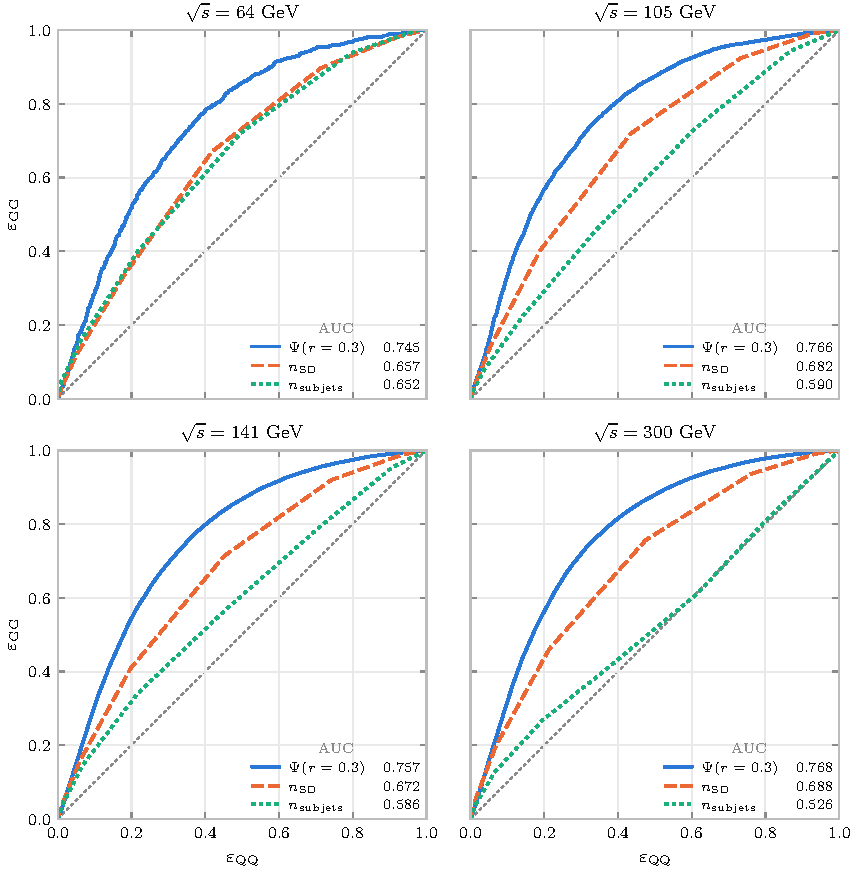
\includegraphics[width=0.94\textwidth]{figures/fig_roc_panels.pdf}
\caption{ROC curves for gluon-versus-quark discrimination at the four
centre-of-mass energies. Signal is jets from GG events, background is jets from QQ
events. All three observables are evaluated on identical jets (anti-$k_T$,
$R = 1.0$, exclusive two-jet, $E_T > 10$~GeV). The dotted diagonal is the
no-discrimination limit. Legend entries give the area under each curve.}
\label{fig:roc_panels}
\end{figure*}

\begin{table}[htbp]
\caption{Area under the ROC curve for the three discriminants, inclusive in
$\eta$.}
\label{tab:auc}
\begin{ruledtabular}
\begin{tabular}{cccc}
$\sqrt{s}$ [GeV] & $\Psi(r=0.3)$ & $n_{\mathrm{SD}}$ & $n_{\mathrm{subjets}}$ \\
\colrule
 64 & 0.745 & 0.657 & 0.652 \\
105 & 0.766 & 0.682 & 0.590 \\
141 & 0.757 & 0.672 & 0.586 \\
300 & 0.768 & 0.688 & 0.526 \\
\end{tabular}
\end{ruledtabular}
\end{table}

\subsection{Trend with centre-of-mass energy}

Figure~\ref{fig:auc_vs_energy} shows the same information against $\sqrt{s}$.
Two things stand out. The integrated jet shape and the iterated soft-drop
multiplicity are both nearly flat across the whole range, moving by only $0.023$
and $0.031$ in AUC between 64 and 300~GeV. The subjet multiplicity does the
opposite: it falls steadily above 64~GeV, from $0.652$ down to $0.526$, and by
the HERA reference energy it is close to useless.

\begin{figure}[tb]
\centering
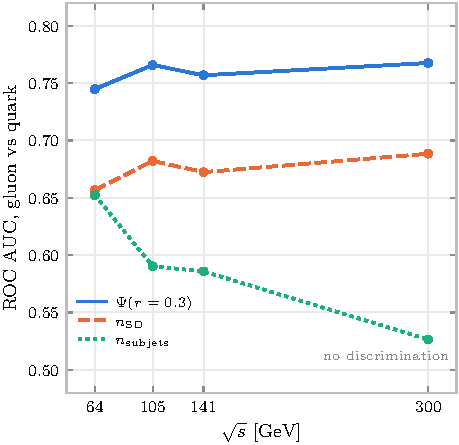
\includegraphics[width=\columnwidth]{figures/fig_auc_vs_energy.pdf}
\caption{Area under the ROC curve as a function of centre-of-mass energy for the
three discriminants, inclusive in $\eta$. The integrated jet shape and the
iterated soft-drop multiplicity are stable across the range; the subjet
multiplicity degrades towards the no-discrimination limit as $\sqrt{s}$ grows.}
\label{fig:auc_vs_energy}
\end{figure}

So the lead of $n_{\mathrm{SD}}$ over $n_{\mathrm{subjets}}$ grows with energy:
the AUC gap is $0.005$ at 64~GeV, $0.092$ at 105~GeV, $0.086$ at 141~GeV and
$0.162$ at 300~GeV. At the lowest EIC energy the two counting observables are
about equally good; by the HERA energy they are not close.

\subsection{Origin of the scale sensitivity}

$n_{\mathrm{subjets}}$ falls off because its resolution threshold is an absolute
scale. In the HERA-300 sample the inclusive means are
$\langle n_{\mathrm{subjets}}\rangle_{\mathrm{QQ}} = 3.10$ and
$\langle n_{\mathrm{subjets}}\rangle_{\mathrm{GG}} = 3.30$, a mean separation of
only $\mathcal{S} = 0.087$ from Eq.~(\ref{eq:sep}). Inside a single
pseudorapidity bin the separation is much better: $\mathcal{S} = 0.657$ for
$\eta \in [-1,0)$, dropping to $0.501$ for $\eta \in [2,3)$. The inclusive number
is not the average of the per-bin ones, because the mean itself slides with
$\eta$ --- from $4.25$ in the most backward bin to $1.63$ in the most forward.

Decomposing the pooled variance into within-bin and between-bin components,
\begin{equation}
\sigma^2_{\mathrm{pool}} \;=\;
\underbrace{\bigl\langle \sigma^2_{\mathrm{bin}} \bigr\rangle_{\mathrm{bins}}}_{\text{within}}
\;+\;
\underbrace{\mathrm{Var}_{\mathrm{bins}}\bigl(\langle X\rangle_{\mathrm{bin}}\bigr)}_{\text{between}},
\end{equation}
puts a number on it. For $n_{\mathrm{subjets}}$ at HERA-300 the between-bin term
is $48.0\%$ of the pooled QQ variance and $62.3\%$ of the pooled GG variance. For
$n_{\mathrm{SD}}$ it is under $0.2\%$ in both classes. So roughly half the width
of the inclusive $n_{\mathrm{subjets}}$ distribution is not class information at
all --- it is the observable following the jet kinematics, dragged in by pooling
over $\eta$. The iterated soft-drop multiplicity, cut on a dimensionless
fraction, picks up almost none of this: its per-bin means agree to within $2\%$
across the full $\eta$ range.

The same argument explains why $n_{\mathrm{subjets}}$ gets worse as $\sqrt{s}$
rises. More energy means a wider spread of jet transverse momenta in the
accepted sample, and the number of emissions above a fixed $p_T^2$ threshold
grows with the jet $p_T$. A wider $p_T$ spread therefore just adds more pooled
width that says nothing about the class.

\subsection{Pseudorapidity binning}\label{sec:etabins}

If the argument above is right, binning in $\eta$ before building the ROC should
give $n_{\mathrm{subjets}}$ most of its discrimination back, and should do almost
nothing to the other two. Figure~\ref{fig:auc_vs_eta} shows that this is exactly
what happens. The dotted horizontal lines are the inclusive values. For
$\Psi(0.3)$ and $n_{\mathrm{SD}}$ the per-bin points sit on those lines. For
$n_{\mathrm{subjets}}$ they sit far above: at HERA-300 it goes from $0.526$
pooled to $0.737$--$0.743$ bin by bin.

\begin{figure*}[t]
\centering
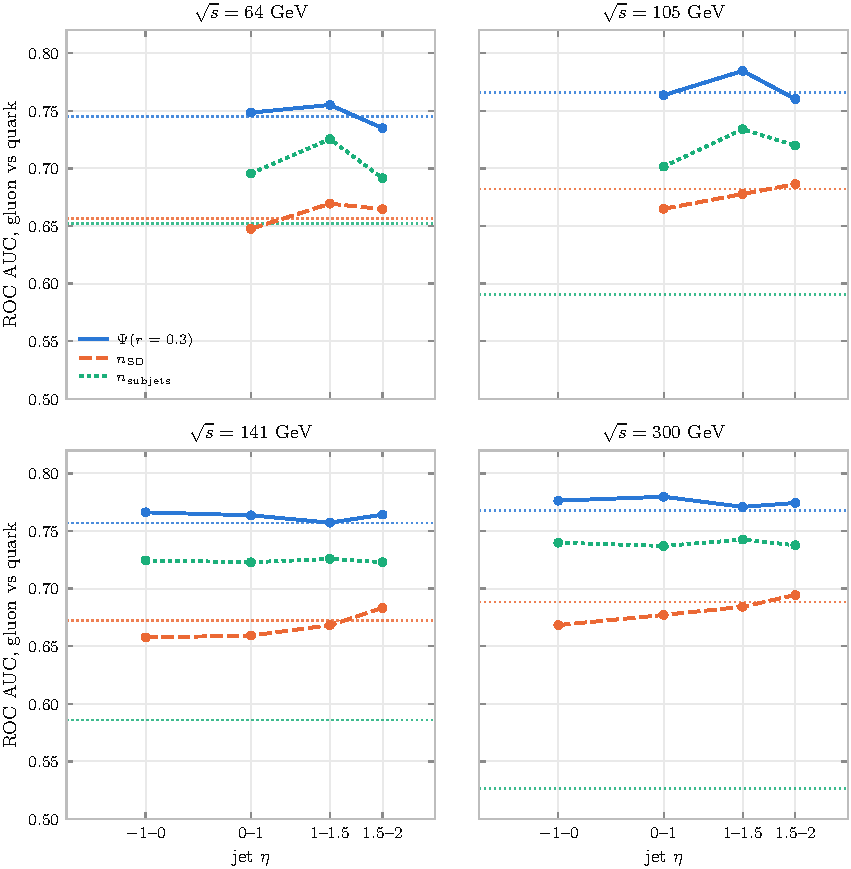
\includegraphics[width=0.94\textwidth]{figures/fig_auc_vs_eta.pdf}
\caption{AUC in each pseudorapidity bin (markers) against the inclusive value for
the same sample (dotted horizontal lines). $\Psi(0.3)$ and $n_{\mathrm{SD}}$ are
unaffected by pooling; $n_{\mathrm{subjets}}$ loses a large amount of
discrimination to it. The $\eta \in [-1,0)$ bin is absent at 64 and 105~GeV,
where the sample has too few jets there.}
\label{fig:auc_vs_eta}
\end{figure*}

This reverses the ordering of the two counting observables. Inclusively
$n_{\mathrm{SD}}$ is ahead at three of the four energies, by up to $0.162$. In
every one of the fourteen $\eta$ bins we can measure, $n_{\mathrm{subjets}}$ is
ahead instead, by between $0.027$ and $0.072$. There is no exception. Which of
the two counting observables looks better is therefore not a property of the
observables on their own: it depends entirely on whether the measurement is
quoted inclusively or differentially.

Since that conclusion could be an artefact of one particular choice of bins, we
repeated the exercise with uniform bins of varying width over a fixed range
$-1 < \eta < 2$, so that the widest case is the genuine pooled limit of the same
jets. Table~\ref{tab:binwidth} and Fig.~\ref{fig:auc_vs_binwidth} give the
jet-weighted mean AUC as the bin width shrinks from $3$ (one bin) to $0.25$
(twelve bins). $\Psi(0.3)$ and $n_{\mathrm{SD}}$ move by no more than $0.007$
across that whole range. $n_{\mathrm{subjets}}$ climbs by $0.055$ at 64~GeV and
by $0.094$ at 300~GeV, rising monotonically as the bins narrow and flattening off
below a width of about $0.5$. It is already ahead of $n_{\mathrm{SD}}$ at a width
of $1.5$ and stays ahead as the bins narrow further; only in the fully pooled
limit does $n_{\mathrm{SD}}$ lead. The effect is therefore not a feature of the
binning we happened to pick. It is controlled by how much jet-kinematic spread
each bin still contains.

\begin{table}[htbp]
\caption{Jet-weighted mean AUC as a function of $\eta$ bin width, for uniform
bins over $-1 < \eta < 2$. A width of $3$ is a single pooled bin. Bins holding
fewer than 100 jets of either class are dropped, which at 64 and 105~GeV removes
most of the narrowest binning; those two entries rest on limited statistics.}
\label{tab:binwidth}
\begin{ruledtabular}
\begin{tabular}{ccccc}
$\sqrt{s}$ [GeV] & width & $\Psi(r=0.3)$ & $n_{\mathrm{SD}}$ & $n_{\mathrm{subjets}}$ \\
\colrule
     & 3.00 & 0.746 & 0.656 & 0.655 \\
  64 & 1.00 & 0.748 & 0.656 & 0.698 \\
     & 0.25 & 0.744 & 0.666 & 0.710 \\
\colrule
     & 3.00 & 0.767 & 0.678 & 0.645 \\
 105 & 1.00 & 0.768 & 0.675 & 0.702 \\
     & 0.25 & 0.767 & 0.671 & 0.725 \\
\colrule
     & 3.00 & 0.758 & 0.668 & 0.641 \\
 141 & 1.00 & 0.763 & 0.665 & 0.714 \\
     & 0.25 & 0.764 & 0.665 & 0.731 \\
\colrule
     & 3.00 & 0.772 & 0.684 & 0.651 \\
 300 & 1.00 & 0.776 & 0.680 & 0.728 \\
     & 0.25 & 0.776 & 0.679 & 0.745 \\
\end{tabular}
\end{ruledtabular}
\end{table}

\begin{figure*}[t]
\centering
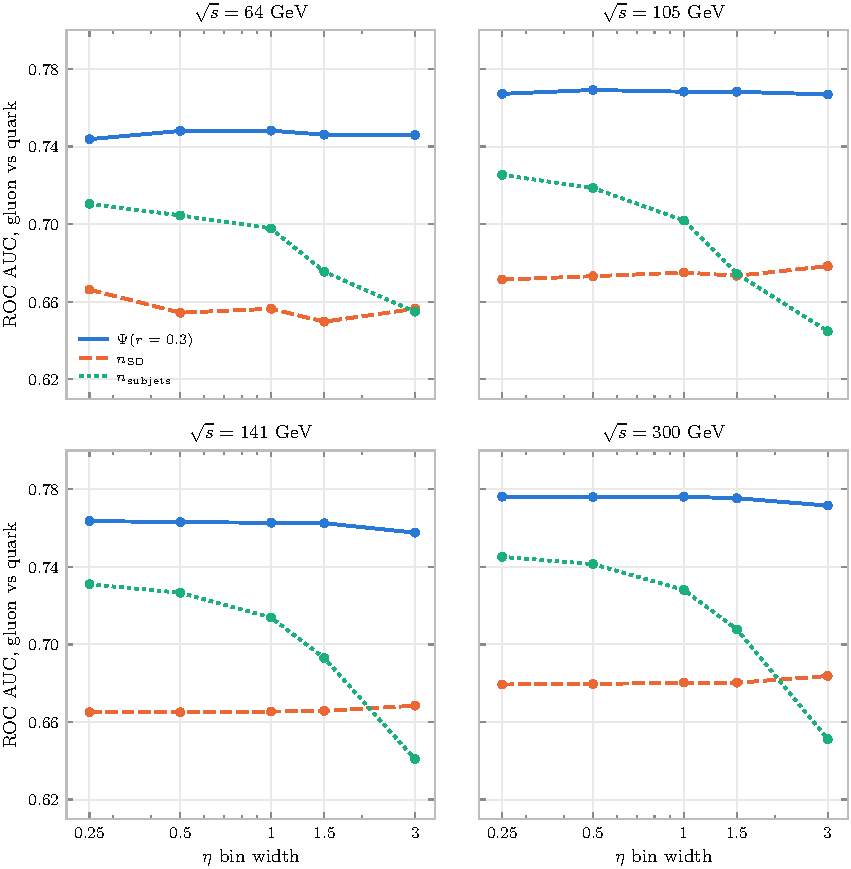
\includegraphics[width=0.94\textwidth]{figures/fig_auc_vs_binwidth.pdf}
\caption{Jet-weighted mean AUC against $\eta$ bin width, for uniform bins over
$-1 < \eta < 2$. A width of $3$ is the pooled limit. $\Psi(0.3)$ and
$n_{\mathrm{SD}}$ are flat; $n_{\mathrm{subjets}}$ rises steadily as the bins
narrow and overtakes $n_{\mathrm{SD}}$ near a width of $1.5$.}
\label{fig:auc_vs_binwidth}
\end{figure*}

$\Psi(0.3)$ is the best of the three either way. It leads in every bin, at every
width, at every energy.

\subsection{Colour-factor content}

At HERA-300 we measure
$\langle n_{\mathrm{SD}}\rangle_{\mathrm{GG}} /
 \langle n_{\mathrm{SD}}\rangle_{\mathrm{QQ}} = 4.41/3.47 = 1.27$, against the
leading-logarithmic expectation $C_A/C_F = 2.25$ of Eq.~(\ref{eq:casimir}). That
is well short of the asymptotic value, and it should be: the LL result assumes
plenty of logarithmic room for primary-branch emissions, while a 10--20~GeV jet
at $z_{\mathrm{cut}} = 0.1$ only has a handful of splittings that qualify. The
counting observable is working far from the regime where its colour-factor
argument is sharp, and that puts a ceiling on what any counting tagger can do in
this kinematic range.

\section{Discussion}\label{sec:discussion}

\subsection{Why the integrated observable wins}

The three observables differ in how much of the jet they use. Both counting
observables boil the jet down to a count of splittings above a threshold. They
throw away everything below it and treat everything above it the same. The
integrated jet shape sets no threshold at all: every constituent counts, in
proportion to its transverse energy, and the radial profile covers hard and soft
emissions alike. When there are only a few splittings above threshold to begin
with --- and Sec.~\ref{sec:results} shows that is the case here --- throwing away
the rest is expensive. The colour-flow information $n_{\mathrm{SD}}$ holds in
discrete form is also in $\Psi(r)$, in continuous form, and at these jet energies
the continuous form keeps more of it.

Robustness is the second reason. Apart from the choice of $r$, $\Psi(r)$ has no
tagging parameter, and $r$ is less a tuning knob than a choice of where to read a
profile you have measured in full. $n_{\mathrm{SD}}$ comes with
$(z_{\mathrm{cut}}, \beta)$ and $n_{\mathrm{subjets}}$ with $y_{\mathrm{cut}}$,
and each of those thresholds interacts with the underlying event and the proton
remnant in ways that have to be pinned down before the tagger can be trusted. For
a first measurement at a facility with no data yet, having fewer such choices to
defend is worth a lot.

\subsection{Implications for EIC measurements}

These results point to a concrete recommendation. For the first round of EIC
jet-substructure measurements, the integrated jet shape is the right choice: it
separates the classes best of the three, it holds up across the full EIC energy
range and matches the HERA reference, it adds no tagging parameters to defend,
and it can be compared directly with the archival ZEUS measurements --- a
validation path no newer observable has.

The choice between the two counting observables is not settled in the abstract:
it follows from how the measurement is presented. If the result is quoted
inclusively in $\eta$, use $n_{\mathrm{SD}}$, which is untouched by pooling and
leads by up to $0.162$ in AUC. If it is quoted differentially, which is the more
natural way to publish, use $n_{\mathrm{subjets}}$, which leads in every bin we
can measure. Section~\ref{sec:etabins} shows that bins of width $1.5$ or narrower
are already enough to put $n_{\mathrm{subjets}}$ ahead.

What should not be done is to quote $n_{\mathrm{subjets}}$ inclusively. Its
discrimination power is real, but pooling over $\eta$ throws most of it away, and
at HERA energies the pooled result is close to no discrimination at all.

\section{Conclusion}\label{sec:conclusion}

We have compared three quark/gluon discriminants --- the integrated jet shape
$\Psi(r=0.3)$, the $k_T$ exclusive subjet multiplicity $n_{\mathrm{subjets}}$,
and the iterated soft-drop multiplicity $n_{\mathrm{SD}}$ --- on the same
anti-$k_T$ jets from PYTHIA~8 photoproduction events at HERA and at the three EIC
design energies. Four things came out of it.

\textit{First}, the integrated jet shape separates gluons from quarks best in
every sample, with ROC AUCs of $0.745$, $0.766$, $0.757$ and $0.768$ at
$\sqrt{s} = 64$, $105$, $141$ and $300$~GeV. The iterated soft-drop multiplicity
follows at $0.66$--$0.69$, and the subjet multiplicity trails at $0.53$--$0.65$.

\textit{Second}, which of the two counting observables is better depends on how
the measurement is binned, and the reason is the difference in their thresholds.
At $\beta = 0$, $n_{\mathrm{SD}}$ counts splittings above a dimensionless
momentum fraction, so it barely notices a change of jet scale.
$n_{\mathrm{subjets}}$ at fixed $y_{\mathrm{cut}}$ counts emissions above an
absolute $p_T^2$ scale, so it also picks up soft wide-angle radiation, and that
contribution grows with the jet $p_T$. Pooled over $\eta$, that extra spread is
pure dilution: splitting the inclusive $n_{\mathrm{subjets}}$ variance into
within- and between-bin parts puts 48--62\% of the HERA-300 pooled variance in
the between-bin term, against under $0.2\%$ for $n_{\mathrm{SD}}$. So
inclusively $n_{\mathrm{SD}}$ wins, by a margin that grows with $\sqrt{s}$ and
reaches $0.162$ at HERA. Bin in $\eta$ and the dilution goes away, and the
ordering reverses: $n_{\mathrm{subjets}}$ leads in all fourteen bins we can
measure, by $0.027$ to $0.072$. A scan over bin width shows
$n_{\mathrm{subjets}}$ already ahead at $\Delta\eta = 1.5$ and staying ahead as
the bins narrow, while $\Psi(0.3)$ and $n_{\mathrm{SD}}$ shift by less than
$0.007$ across the entire scan.

\textit{Third}, the integrated jet shape wins because it uses the whole radial
energy distribution, hard splittings and soft ones alike, instead of counting
only what clears a threshold. The colour-flow information $n_{\mathrm{SD}}$
carries in discrete form is in $\Psi(r)$ too, in continuous form. And because
$\Psi(r)$ has no internal cutoff, it is less exposed to the underlying event and
the proton remnant in the low-$p_T$ regime that EIC photoproduction lives in.

Taken together, this is why we would put $\Psi(r=0.3)$ forward as the headline
discriminant for the first round of EIC jet-substructure measurements: it keeps
the number of tagging parameters to a minimum and it can be compared directly
with the published HERA-ZEUS data. $n_{\mathrm{SD}}$ is the natural follow-up,
especially once there is real data to calibrate against and enough of it to tune
an operating point. We hope what we have done here is useful to the EIC
programme in two ways: as a benchmark for comparing taggers, and as the
generator-level baseline that detector systematics can later be quoted against.

\appendix

\section{Supplementary material}\label{sec:appendix}

\subsection{ROC curves in individual pseudorapidity bins}

Section~\ref{sec:etabins} quotes per-bin areas but shows the curves only in
aggregate. Figures~\ref{fig:app_roc_300} and \ref{fig:app_roc_64} give the
underlying ROC curves bin by bin, at the highest and lowest energies in the
study. The reversal discussed in the main text is visible directly: in every
panel the $n_{\mathrm{subjets}}$ curve lies above the $n_{\mathrm{SD}}$ curve,
the opposite of what the pooled measurement in Fig.~\ref{fig:roc_panels} shows.

At $\sqrt{s} = 64$~GeV only three bins are shown. The sample has just ten GG
jets with $\eta \in [-1,0)$, too few for a meaningful ROC, so that bin is
dropped; the corresponding QQ count is 690. All four bins are usable at
$\sqrt{s} = 300$~GeV.

\begin{figure*}[t]
\centering
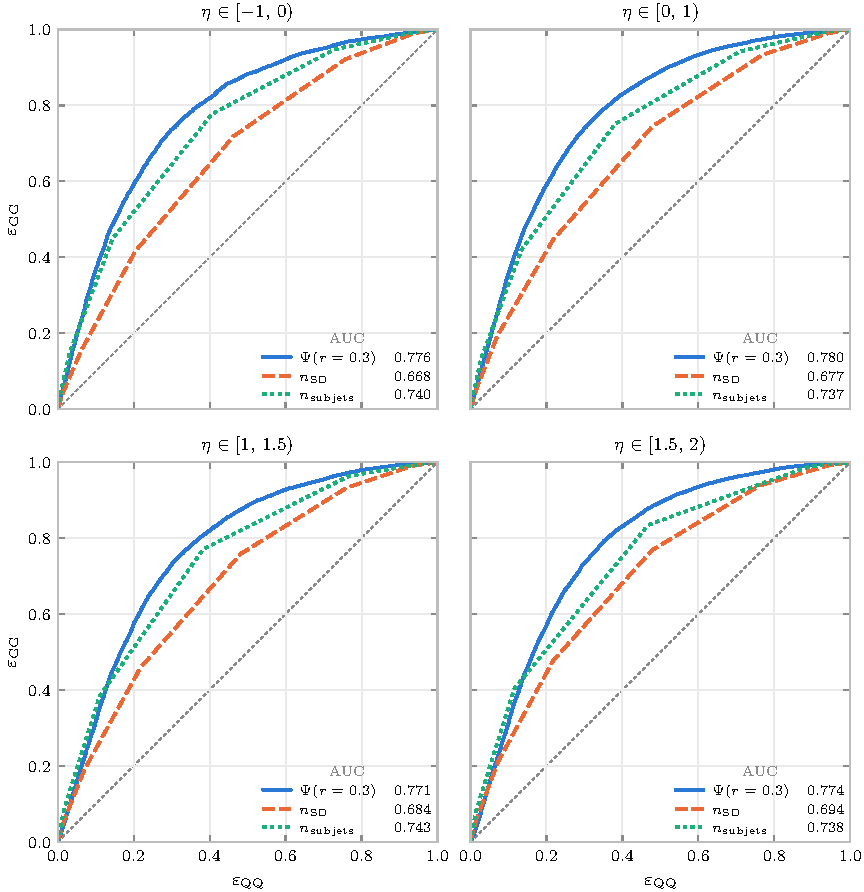
\includegraphics[width=0.94\textwidth]{figures/fig_app_roc_eta_300.pdf}
\caption{ROC curves in each pseudorapidity bin at $\sqrt{s} = 300$~GeV. Signal
is jets from GG events, background is jets from QQ events. Jets are binned
individually by their own $\eta$. Legend entries give the area under each
curve.}
\label{fig:app_roc_300}
\end{figure*}

\begin{figure*}[t]
\centering
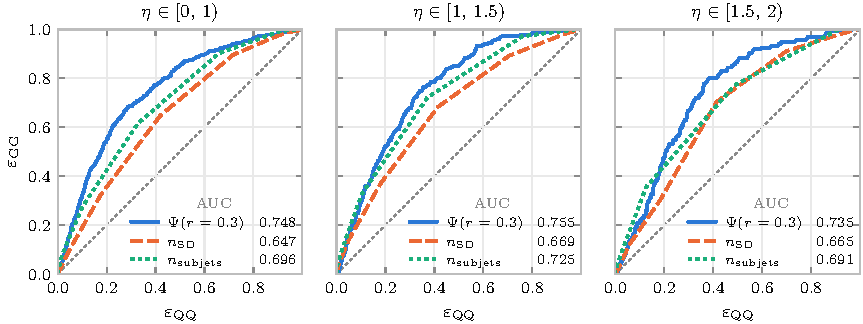
\includegraphics[width=0.94\textwidth]{figures/fig_app_roc_eta_64.pdf}
\caption{As Fig.~\ref{fig:app_roc_300}, at $\sqrt{s} = 64$~GeV. The
$\eta \in [-1,0)$ bin is omitted: it holds only ten GG jets.}
\label{fig:app_roc_64}
\end{figure*}

\subsection{Jet counts per pseudorapidity bin}

Table~\ref{tab:jetcounts} lists how many jets enter each bin. Jets are counted
individually, not as events: a dijet event contributes its two jets to
whichever bins their own pseudorapidities fall in, and the two need not be the
same bin. The bins are half-open, $[\eta_{\min}, \eta_{\max})$, so they tile
the range $-1 \le \eta < 2$ exactly. The per-bin counts therefore sum to the
total over that range with no jet lost and none counted twice, as the closure
row shows.

The inclusive row is larger because it covers the full acceptance
$-4 < \eta < 4$ used for the pooled results of Sec.~\ref{sec:results}. The
difference is jets forward of $\eta = 2$, which fall outside the binned range:
at $\sqrt{s} = 300$~GeV these account for $29\%$ of the QQ jets and $44\%$ of
the GG jets. This is worth keeping in mind when comparing the per-bin markers
of Fig.~\ref{fig:auc_vs_eta} with its inclusive reference lines, since the two
are evaluated over different $\eta$ ranges.

\begin{table}[htbp]
\caption{Jet counts per pseudorapidity bin. ``Sum of bins'' is the total over
the four bins; ``total'' is a direct count over $-1 \le \eta < 2$. The two
agree exactly at every energy. ``Inclusive'' is the full acceptance
$-4 < \eta < 4$.}
\label{tab:jetcounts}
\begin{ruledtabular}
\begin{tabular}{llrr}
$\sqrt{s}$ [GeV] & bin & $N_{\mathrm{QQ}}$ & $N_{\mathrm{GG}}$ \\
\colrule
    & $[-1, 0)$    &  \phantom{0}\phantom{0}690 & \phantom{00}10 \\
    & $[0, 1)$     &  7\,927 &   340 \\
 64 & $[1, 1.5)$   &  4\,014 &   252 \\
    & $[1.5, 2)$   &  2\,065 &   135 \\
    & sum of bins  & 14\,696 &   737 \\
    & total        & 14\,696 &   737 \\
    & inclusive    & 15\,132 &   758 \\
\colrule
    & $[-1, 0)$    &    617 &    16 \\
    & $[0, 1)$     &  8\,295 &   601 \\
105 & $[1, 1.5)$   &  5\,642 &   612 \\
    & $[1.5, 2)$   &  5\,131 &   679 \\
    & sum of bins  & 19\,685 & 1\,908 \\
    & total        & 19\,685 & 1\,908 \\
    & inclusive    & 25\,258 & 2\,796 \\
\colrule
    & $[-1, 0)$    & 20\,036 & 1\,538 \\
    & $[0, 1)$     & 50\,776 & 6\,634 \\
141 & $[1, 1.5)$   & 24\,329 & 4\,735 \\
    & $[1.5, 2)$   & 19\,555 & 4\,612 \\
    & sum of bins  & 114\,696 & 17\,519 \\
    & total        & 114\,696 & 17\,519 \\
    & inclusive    & 135\,800 & 22\,930 \\
\colrule
    & $[-1, 0)$    & 22\,897 & 4\,003 \\
    & $[0, 1)$     & 37\,961 & 11\,283 \\
300 & $[1, 1.5)$   & 18\,660 & 7\,965 \\
    & $[1.5, 2)$   & 16\,487 & 8\,739 \\
    & sum of bins  & 96\,005 & 31\,990 \\
    & total        & 96\,005 & 31\,990 \\
    & inclusive    & 134\,774 & 57\,592 \\
\end{tabular}
\end{ruledtabular}
\end{table}

\bibliography{EIC_Observables}

\end{document}